\documentclass{../bredelebeamer}
\usepackage{multirow}
\usepackage{pdfpages}
\usepackage{braket,bigstrut}
\usepackage{palatino}
\usepackage{multicol,bigstrut}
\usepackage{listings}
\usepackage{tikz}
\usepackage{pgfplots}
\pgfplotsset{compat=1.17}
\usepackage{booktabs}
\usepackage{amsmath,amssymb,amsfonts,cancel,physics,siunitx}
\usetikzlibrary{positioning,shadows,backgrounds,calc}%
\setbeamercolor{footnote mark}{fg=black}
\setbeamercolor{footnote}{fg=black}


\renewcommand{\baselinestretch}{0.9}

\usepackage[backend=bibtex8,style=authortitle,autocite=footnote]{biblatex}
%\addbibresource{../../references.bib}

\renewbibmacro*{cite:title}{%
	\printtext[bibhyperref]{%
		\printfield[citetitle]{labeltitle}%
		\setunit{\space}%
		\printtext[parens]{\printdate}%
	}%
}

\renewcommand{\figurename}{{\bf Fig.}}
\usefonttheme{serif} % default family is serif

\renewcommand{\baselinestretch}{0.9}

\title[$U(1)_{T^3R}$ - PUCP 2025]{Probing light scalars and vector-like quarks at the high-luminosity LHC}
\subtitle{}
\author[Cristian F. Rodríguez]{
	$ $\\
	Cristian Fernando Rodríguez Cruz\\
	$ $\\
	$ $\\
	$ $\\
	$ $\\
	Authors:\\
	A. Flórez\inst{1}, \textcolor{Framableu}{\textbf{C. Rodriguez}}\inst{1},  \\
	%J. Peñuela-Parra\inst{1},\\
	% J. Jones-Pérez\inst{2}, \\
	A. Gurrola\inst{2},
	U. S. Qureshi\inst{2},
}

\institute[Uniandes]{%
    \inst{1} Universidad de los Andes\and
    \inst{2} Vanderbilt University
}
\date{\today}
\lstset{language=C++,
  basicstyle=\ttfamily,
  keywordstyle=\color{blue}\ttfamily,
  stringstyle=\color{red}\ttfamily,
  commentstyle=\color{green}\ttfamily,
  morecomment=[l][\color{magenta}]{\#}
}

\begin{document}
\frame{\titlepage}

\begin{frame}
    \frametitle{Outline}
    \tableofcontents
\end{frame}

\section{Motivation}

\begin{frame}{The Standard Model of Particle Physics}
        \begin{center}
            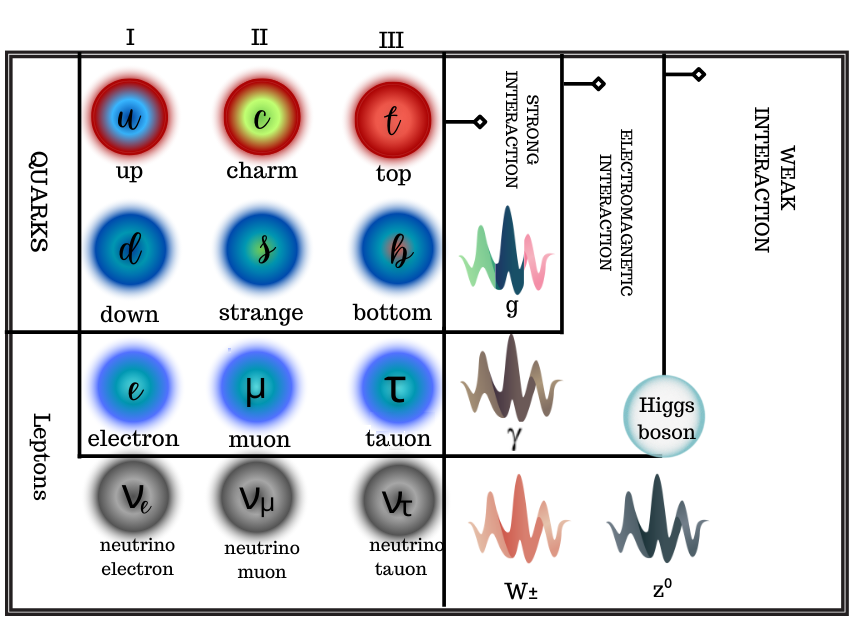
\includegraphics[width=.9\linewidth]{../2023_paper/SM}
        \end{center}
\end{frame}

\subsection{$B-L$ Symmetry}
\begin{frame}{Standard Model Charges (1 Generation)}{}
{

\footnotesize
SM is free of gauge anomalies, which are cancellations of gauge charges in fermion loops. And has two accidental global symmetries: \(U(1)_B\) and \(U(1)_L\).
\begin{table}[h]
\centering
\begin{tabular}{|c|c|c|c|c|c|c|c|c|}
\hline
\textbf{Fermion} & \boldmath\(SU(3)_c\) & \boldmath\(SU(2)_L\) & \boldmath\(B\) & \boldmath\(L\) & \boldmath\(Y\) & \boldmath\(Q\) & \boldmath\(B-L\) & \boldmath\(T^3_L\) \bigstrut \\ \hline
\hline
\(\nu_{eL}\)     & \textbf{1}       & \textbf{2}       & 0    & +1   & -1    & 0      & -1     & +\(\frac{1}{2}\)  \bigstrut \\ \hline
\(e_L\)          & \textbf{1}       & \textbf{2}       & 0    & +1   & -1    & -1     & -1     & -\(\frac{1}{2}\)  \bigstrut \\ \hline
\hline
\(u_L\)          & \textbf{3}       & \textbf{2}       & \(\frac{1}{3}\) & 0 & \(\frac{1}{3}\) & \(\frac{2}{3}\) & \(\frac{1}{3}\) & +\(\frac{1}{2}\)  \bigstrut \\ \hline
\(d_L\)          & \textbf{3}       & \textbf{2}       & \(\frac{1}{3}\) & 0 & \(\frac{1}{3}\) & \(-\frac{1}{3}\) & \(\frac{1}{3}\) & -\(\frac{1}{2}\)  \bigstrut \\ \hline
\hline
\(e_R\)          & \textbf{1}       & \textbf{1}       & 0    & +1   & -2    & -1     & -1     & 0 \bigstrut \\ \hline
\hline
\(u_R\)          & \textbf{3}       & \textbf{1}       & \(\frac{1}{3}\) & 0 & \(\frac{4}{3}\) & \(\frac{2}{3}\) & \(\frac{1}{3}\) & 0 \bigstrut \\ \hline
\hline
\(d_R\)          & \textbf{3}       & \textbf{1}       & \(\frac{1}{3}\) & 0 & \(-\frac{2}{3}\) & \(-\frac{1}{3}\) & \(\frac{1}{3}\) & 0 \bigstrut \\ \hline
\end{tabular}
\end{table}

Could we extend the SM with a new \(U(1)\) gauge symmetry related to the accidental global symmetries \(U(1)_B\) and \(U(1)_L\)?
\begin{table}[h]
\centering
\begin{tabular}{|c|c|c|c|}
\hline
\textbf{Group Symmetry} & \boldmath$[SU(3)_c]^2 U(1)$ & \boldmath$[SU(2)_L]^2 U(1)$ & \textbf{Anomaly-Free?} \bigstrut \\ \hline
\boldmath$U(1)_B$       & $1 \neq 0$                  & $1 \neq 0$                  & No \bigstrut \\ \hline
\boldmath$U(1)_L$       & $0$                         & $1 \neq 0$                  & No \bigstrut \\ \hline
\boldmath$U(1)_{B-L}$   & $0$                         & $0$                         & Yes -> could be gauge symmetry\bigstrut \\ \hline
\end{tabular}
\end{table}

}
\end{frame}
\begin{frame}{A possible explanation for the hypercharge of SM fermions}{}
	From the EWSB point of view, where the EM gauge group is a subgroup of the electroweak gauge group, which breaks down from \(SU(2)_L \times U(1)_Y\) to \(U(1)_{\text{EM}}\).

	In SM the electric charge is given by the Gell-Mann-Nishijima formula:
	\begin{equation}
	\hat Q_{\text{EM}} = \hat T^3_{\text{L}} + \frac{\hat Y}{2}
	\end{equation}
	where $T^3_{\text{L}}$ is the third component of the weak isospin $SU(2)_L$ and $Y$ is the hypercharge of the $U(1)_Y$ gauge group.
	
	For example, for the left-handed electron component:
	\begin{equation}
	\hat Q_{\text{EM}}(e_L) = \hat T^3_{\text{L}}(e_L) + \frac{\hat Y(e_L)}{2} = \left(-\frac{1}{2} - \frac{1}{2}\right) e_L = (-1) e_L
	\end{equation}
	$Y$ values seem arbitrary in SM. Can $Y$ emerge from deeper principles and recover some chiral structure?

	If we use the same isospin values for the left-handed fermions, for the right-handed fermions but as a new symmetry \(U(1)_{T^3_R}\), we can write the following relation:
	\begin{equation}
	\hat Y = 2\hat T^3_{\text{R}} + \frac{\hat B - \hat L}{2}
	\end{equation}
	and the electric charge is given by:
	\begin{equation}
	\hat Q_{\text{EM}} = \hat T^3_{\text{L}} + \hat T^3_{\text{R}} + \frac{\hat B - \hat L}{4}
	\end{equation}
\end{frame}
\section{The $U(1)_{T^3_R}$ Gauge Symmetry}

\begin{frame}{The challenge of the $U(1)_{T^3_R}$ Gauge Symmetry}{Add a $U(1)_{T^3_R}$ gauge add a lot of complications: }
	\begin{itemize}
		\item Which is the origin of the hyptercharge of the Higgs doublet? 
		\begin{equation}
			\hat Y = 2\hat T^3_{\text{R}} + \frac{\hat B - \hat L}{2} + \hat Q_G
		\end{equation}
		
		

		A dark sector or discard the connection between the hypercharge and the new gauge symmetry is needed.

		\vfill 
		\hrule\hrule
		\begin{center}
			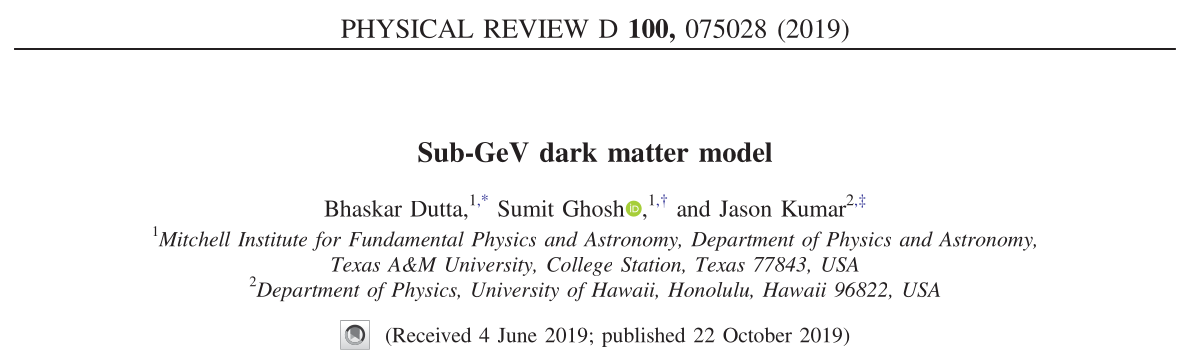
\includegraphics[width=\textwidth]{dutta2019.png}
		\end{center}
	\end{itemize}
\end{frame}

\begin{frame}{Add a $U(1)_{T^3_R}$ gauge add a lot of complications: }
	\begin{itemize}
		\item  A new gauge boson is needed, and it is not near to the electroweak scale.
		$$
			m_V \propto g_V
		$$
		It could be a dark photon with small mass and coupling, or a $Z'$ boson with mass in the TeV range.
		\vfill 
		\begin{center}
			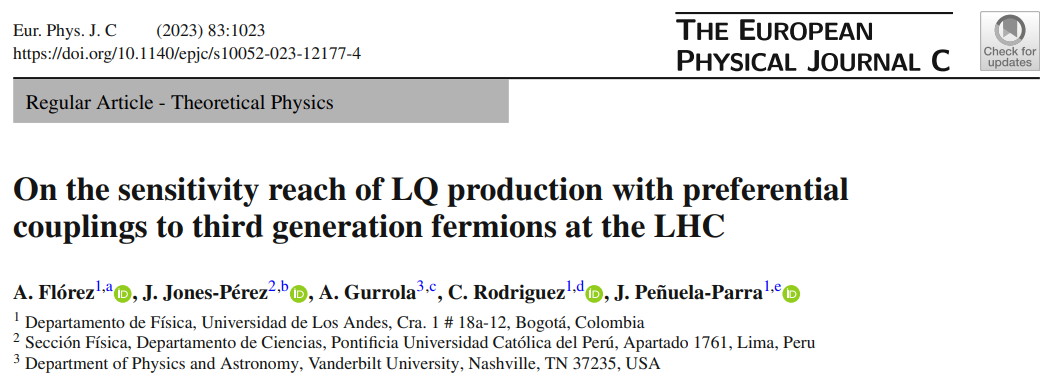
\includegraphics[width=.8\textwidth]{florez2023.png}
		\end{center}
		\hrule\hrule
		\begin{center}
			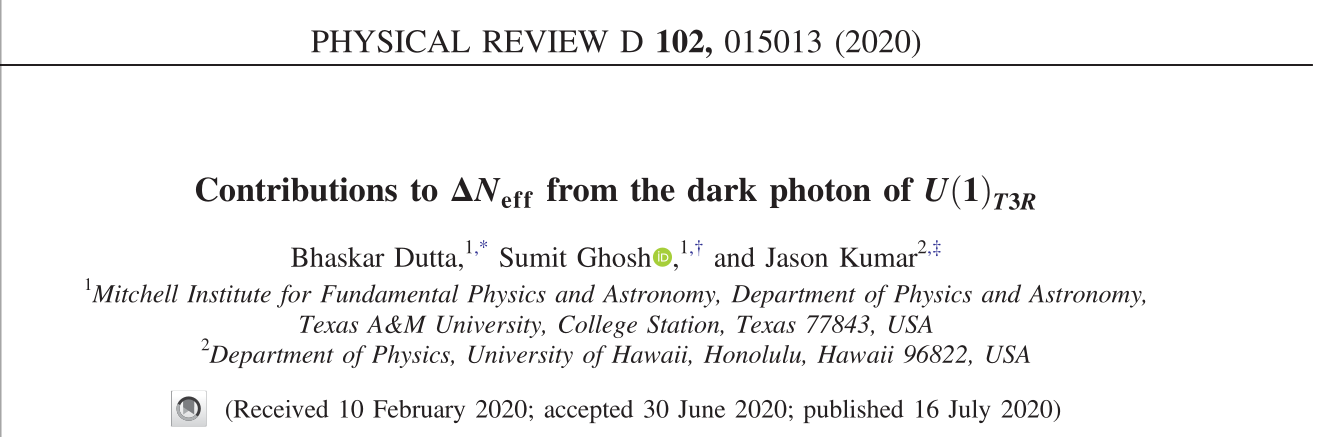
\includegraphics[width=.7\textwidth]{dutta2020b.png}
		\end{center}
	\end{itemize}
\end{frame}

\begin{frame}{A new electroweak symmetry breaking scale is needed, a new scalar $\phi$ is needed.}

		\begin{equation}
    \begin{aligned}
        \mathcal V(\phi,H)
				&= \mu_H^2 H^{\dagger} H 
				+\mu_\phi^2 \phi^* \phi
				\\
				&+\lambda\left(H^{\dagger} H\right)\left(\phi^* \phi\right)
				+\lambda_H\left(H^{\dagger} H\right)^2
				+\lambda_\phi\left(\phi^* \phi\right)^2.
				\end{aligned}
		\end{equation}
		\pause
		Both scalars have independent vacuum expectation values (VEVs), $\expval{H}=v_h/\sqrt2$ and $\expval\phi =v_\phi/\sqrt2$, allowing us to express the doublet and singlet Higgs fields, following a Kibble parametrization, as 
		\begin{align}
				H & = \begin{pmatrix}
						G_{+} \\
						\frac{1}{\sqrt{2}}\left(v_h+\rho_0+i G_{0}\right)
				\end{pmatrix}\label{eq:higgskibblepara1}
				\\
				\phi & =\frac{1}{\sqrt{2}}\left(v_\phi + \rho_\phi+i G_{\phi}\right). \label{eq:higgskibblepara2}
		\end{align}
		\pause
		This give us a matrix mass term for the scalar fields:
		\begin{equation}
			m_{m H}=\left(\begin{array}{cc}
			2 \lambda_H v_h^2 & \lambda_{\phi h}  v_h v_\phi \\
			\lambda v_h v_\phi & 2 \lambda_\phi v_\phi^{ }
			\end{array}\right)
		\end{equation}
		\pause
		The $\rho_h$ and $\rho_\phi$ are an orthogonal mixture of the SM Higgs boson and the dark Higgs
		\begin{equation}
				\begin{pmatrix}
						h
						\\
						\phi'
				\end{pmatrix}
				=
				\begin{pmatrix}
						\cos\alpha & -\sin\alpha
						\\
						\sin\alpha & \cos\alpha
				\end{pmatrix}
				\begin{pmatrix}
						\rho_0
						\\
						\rho_\phi
				\end{pmatrix},
		\end{equation}
		that results from the diagonalization of the mass matrix.	
\end{frame}

\begin{frame}%{$U(1)_{T^3_R}$ is not anomaly-free with only the SM fermions.}
	We need to add right-handed neutrinos
	\begin{table}[h]
    \centering
    \begin{tabular}{ccccc}
    \hline
    \hline
        Field & $SU(3)_C$  & $SU(2)_L$ & $U(1)_Y$ & $U(1)_{T^3_R}$ \\
    \hline\hline
        $q_L$                    & \bf{3} & \bf{2} & 1/6 & 0\\
        $\ell_L$                 & \bf{1} & \bf{2} & -1/2 & 0\\
        $H$                         & \bf{1} & \bf{2} & 1/2 & 0\\
        \hline
        $u_R^{  c}$          & \bf{3} & \bf{1} & -2/3 & -1\\
        $d_R^{  c}$          & \bf{3} & \bf{1} & 1/3 & 1\\
        $\ell_R^{  c}$       & \bf{1} & \bf{1} & 1 & 1\\
        $\nu_R^{  c}$        & \bf{1} & \bf{1} & 0 & -1\\
        $\phi$                      & \bf{1} & \bf{1} & 0 & 1\\
        % \hline
        % $\chi_{u_L}'$               & \bf{3} & \bf{1} & 2/3 & 0\\
        % $\chi_{u_R}^{  c}$     & \bf{3} & \bf{1} & -2/3 & 0\\
        % $\chi_{d_L}'$               & \bf{3} & \bf{1} & -1/3 & 0\\
        % $\chi_{d_R}^{  c}$     & \bf{3} & \bf{1} & 1/3 & 0\\
        % $\chi_{\ell_L}'$            & \bf{1} & \bf{1} & -1 & 0\\
        % $\chi_{\ell_R}^{  c}$  & \bf{1} & \bf{1} & 1 & 0\\
        % $\chi_{\nu_L}'$             & \bf{1} & \bf{1} & 0 & 0\\
        % $\chi_{\nu_R}^{  c}$   & \bf{1} & \bf{1} & 0 & 0\\
    \hline
    \hline
    \end{tabular}
    % \caption{Minimal field content of the model and their representations under the SM and $U(1)_{T^3_R}$ gauge groups.}
    % \label{tab:QMnumbers}
\end{table}
\pause
The SM yukawa couplings are not invariant under the new symmetry,
\begin{equation}
\mathcal{L}_{\text{Yukawa}} = 
\underbrace{-y_e \bar{L}_L \Phi e_R}_{\text{Lepton Yukawa}}
\; + \;
\underbrace{-y_d \bar{Q}_L \Phi d_R}_{\text{Down quark Yukawa}}
\; + \;
\underbrace{-y_u \bar{Q}_L \tilde{\Phi} u_R}_{\text{Up quark Yukawa}}
\; + \; \text{h.c.}
\end{equation}
so $y_u=y_d=y_e=0$ is mandatory. So the masses of the SM fermions are generated by a new mechanism.
\end{frame}
\begin{frame}{{The Universal Seesaw Mechanism}}
	
	They acquire mass from the mixture with a vector-like fermion $\chi_f$, which is charged as the right-handed component of the respective SM fermion, in a UV complete theory. 
	\vfill 
	The terms in the Lagrangian density that contribute to the mass of physical fermions are,
\begin{equation}
    \begin{aligned}
        -\mathcal{L}&\supset 
    Y_{f_L} \bar{f}_L' \chi_{fR}' H 
    +Y_{f_R} \bar\chi_{fL}' f'_R  \phi^* 
    + m_{\chi_f'} \bar{\chi}_{f L}' \chi_{f R}'\\
&+\text { h.c.}
    \end{aligned}
\end{equation}
Therefore, in the vacuum, the mass matrix is
\begin{equation}
    M_f=
    \begin{pmatrix}
    0 & Y_{f_L} v_h /\sqrt2\\
    Y_{f_R} v_\phi /\sqrt2 & m_{\chi_f'}    
    \end{pmatrix}.
\end{equation}

The left- and right-handed components of the physical fermions $(f,\,\chi_f)$ are given by two rotations $\mathcal R(\theta_{f_{L,R}})$ as, 
\begin{equation}
    \begin{pmatrix}
        f_{L,R}
        \\
        \chi_{f_{L,R}}
    \end{pmatrix}
    =
    \begin{pmatrix}
        \pm\cos\theta_{f_{L,R}} & \mp \sin \theta_{f_{L,R}}
        \\
        \sin \theta_{f_{L,R}} & \cos\theta_{f_{L,R}}
    \end{pmatrix}
    \begin{pmatrix}
        f_{L,R}'
        \\
        \chi_{f_{L,R}}'
    \end{pmatrix},
\end{equation}
in a way that $\mathcal{R}(\theta_{f_L})M_f\mathcal{R}^{-1}(\theta_{f_R})=\text{diag}(m_f,m_{\chi_f})$ up to a phase.

\end{frame}

\begin{frame}{{The Universal Seesaw Mechanism}}
	The Yukawa interactions of the physical fermions with the scalar bosons have the form
\begin{equation}
    -\mathcal{L}_{\text{yuk}} 
    = h \bar\psi_{f_L} \mathcal{Y}_{h}\psi_{f_R} + \phi' \bar\psi_{f_L} \mathcal{Y}_{\phi}\psi_{f_R},
\end{equation} 
with $\psi_{f} = (f,\chi_{f})^T$, and the matrices $\mathcal{Y}_{f_{L,R}}$ given by
\begin{align}
    \mathcal{Y}_{h} &= \frac{1}{\sqrt{2}}
    \mathcal{R}(\theta_{f_L})
    \left(
        Y_{f_L}\sigma_+ \cos\alpha 
    - 
    Y_{f_R}\sigma_-\sin\alpha
    \right)
    \mathcal{R}^{-1}(\theta_{f_R})\label{eq:YukawaL}
    \\
    \mathcal{Y}_{\phi} &= \frac{1}{\sqrt{2}}
    \mathcal{R}(\theta_{f_L})
    \left(
    Y_{f_L}\sigma_+ \sin\alpha
    +
    Y_{f_R}\sigma_-\cos\alpha
    \right)
    \mathcal{R}^{-1}(\theta_{f_R}),\label{eq:YukawaR}
\end{align}
where $\sigma_{\pm}=(\sigma_1\pm i\sigma_2)/2$ are the ladder Pauli matrices.


So, you have new vertex like 
\begin{center}
	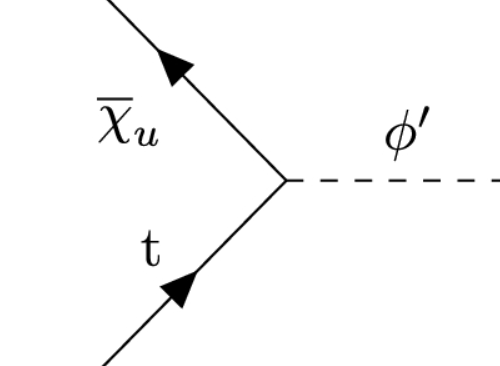
\includegraphics[height=0.3\textheight]{seesaw.png}
\end{center}
\end{frame}

\begin{frame}{Large Hadron Collider}{How can we test the leptoquark hypothesis?}
	\begin{minipage}{.55\linewidth}
		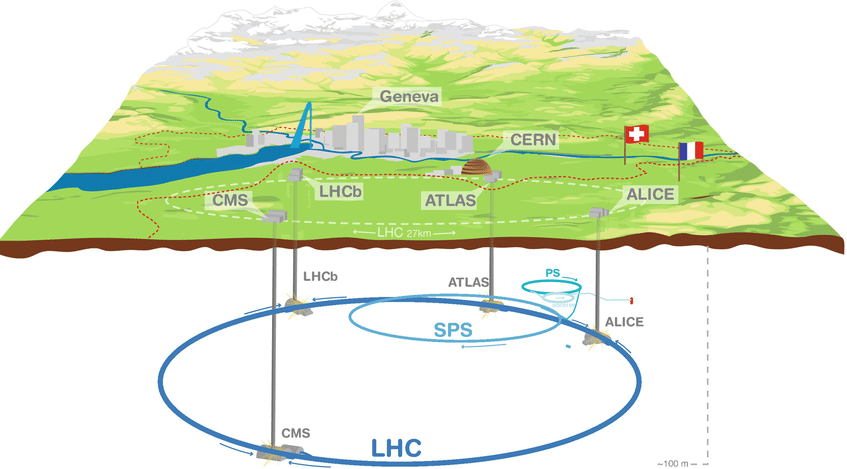
\includegraphics[width=.99\linewidth]{../2023_paper/LHC.png}
	\end{minipage}
	\begin{minipage}{.42\linewidth}
		\begin{itemize}
			\item A Feasibility Study is needed.
			$$ $$
			\item Take Care on the dependence on the different parameters.
			$$ $$
			\item Take care on the content of particles.
			$$ $$
			\item Take care of the signal composition.$$ $$
			\item Take care on interference effects.
		\end{itemize}
	\end{minipage}
\end{frame}

\begin{frame}{Montecarlo Generators}
	

	\begin{center}
		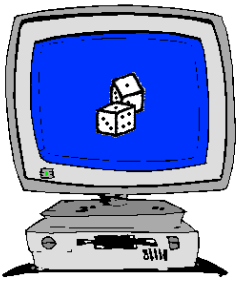
\includegraphics[scale=0.5]{../2023_paper/A1}
	\end{center}

	Useful to predict what we expect to see under certain conditions:
	\begin{itemize}
		\item To perform studies before having the data
		\item To compute event selection efficiency/acceptance
		\item  To predict the ammount and composition of background events
		\item To distinguish different signals. 
	\end{itemize}
	
\end{frame}

\begin{frame}{Feynrules}
	\begin{center}
		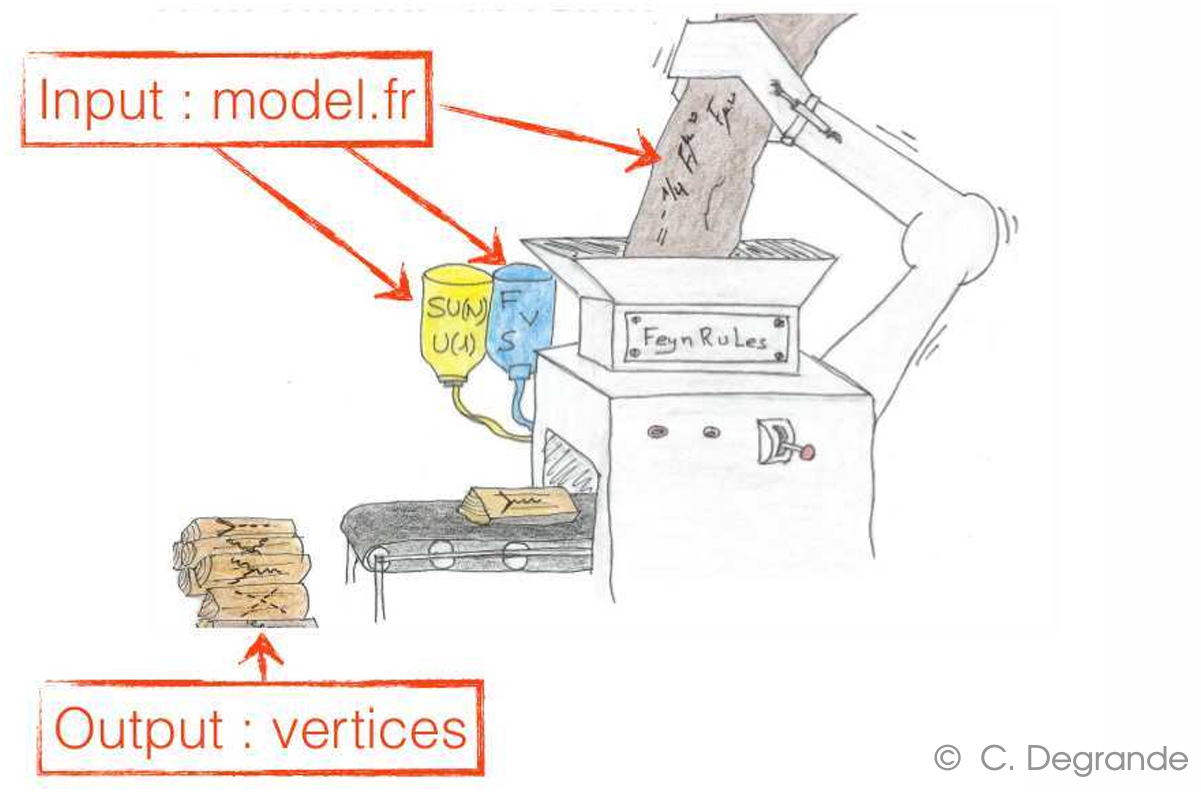
\includegraphics[width=.99\linewidth]{../2023_paper/Feynrules.png}
	\end{center}
\end{frame}

\begin{frame}{Madgraph-Pythia8-Delphes for the LHC}
	\begin{center}
		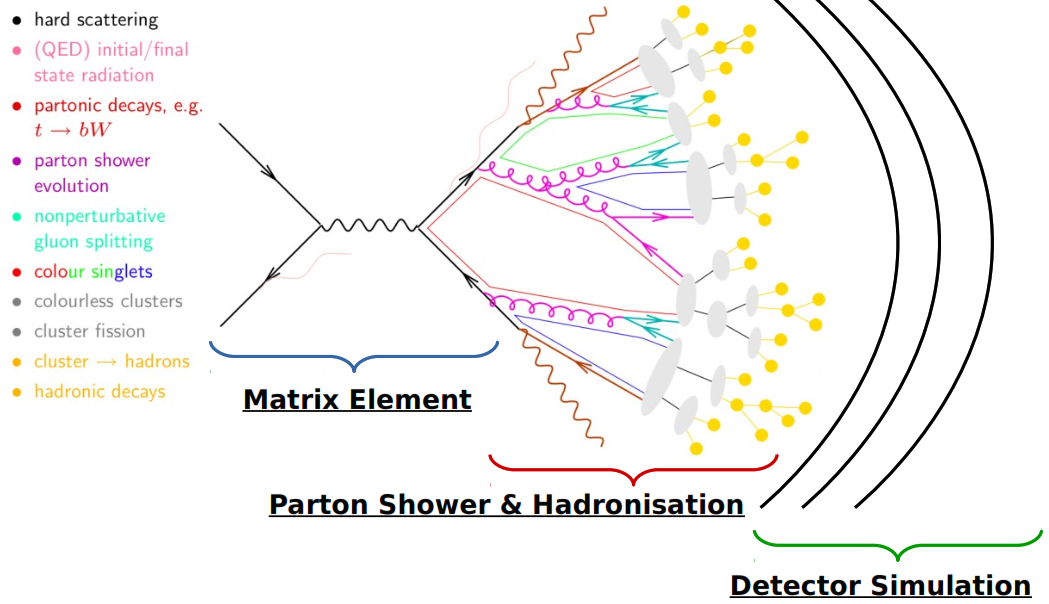
\includegraphics[width=.99\linewidth]{../2023_paper/Madgraph.png}
	\end{center}
\end{frame}


\begin{frame}{Feasibility Studies Workflow}
	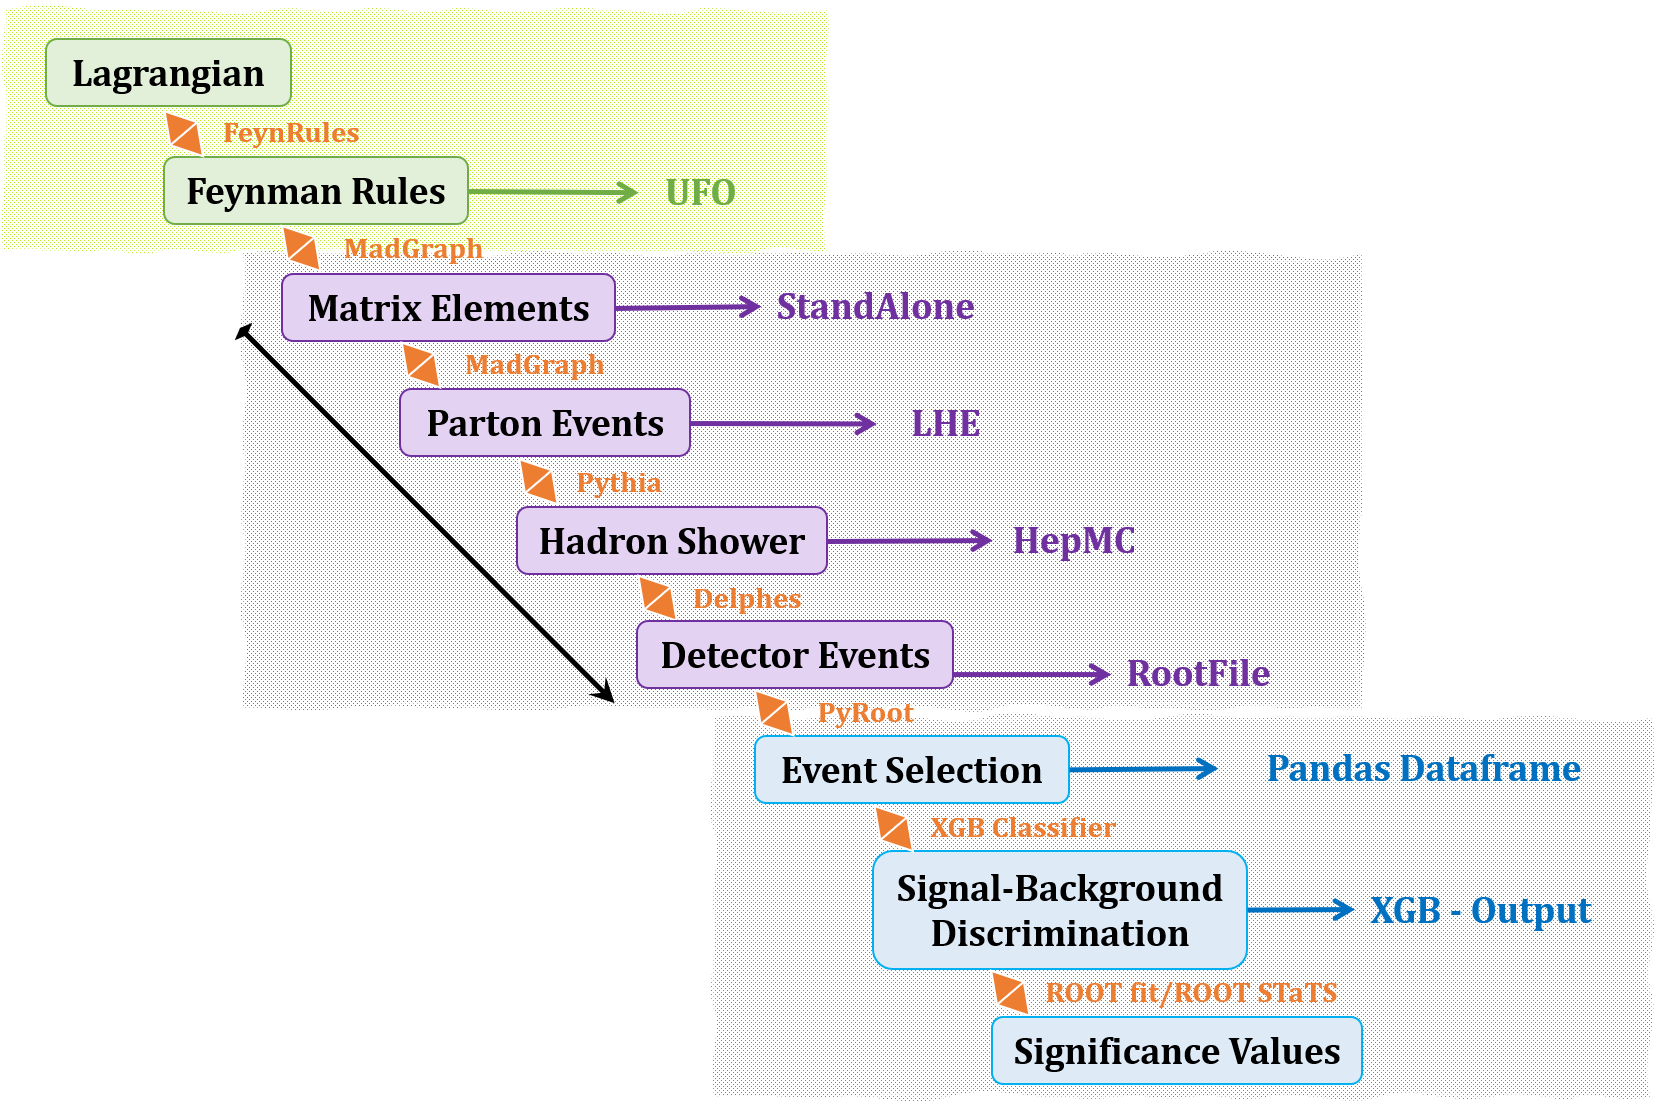
\includegraphics[width=1.0\linewidth]{../2023_paper/Workflow.png}
\end{frame}


\section{Experimental Signatures}
\begin{frame}{Feasible Experimental Signatures}{Search Channel}
	Representative Feynman diagram for the production of a $\phi'$ boson in association with a $\chi_\mathrm{u}$ vector-like quark through the fusion of a top quark and $\chi_\mathrm{u}$ vector-like quark. 
	\begin{center}
		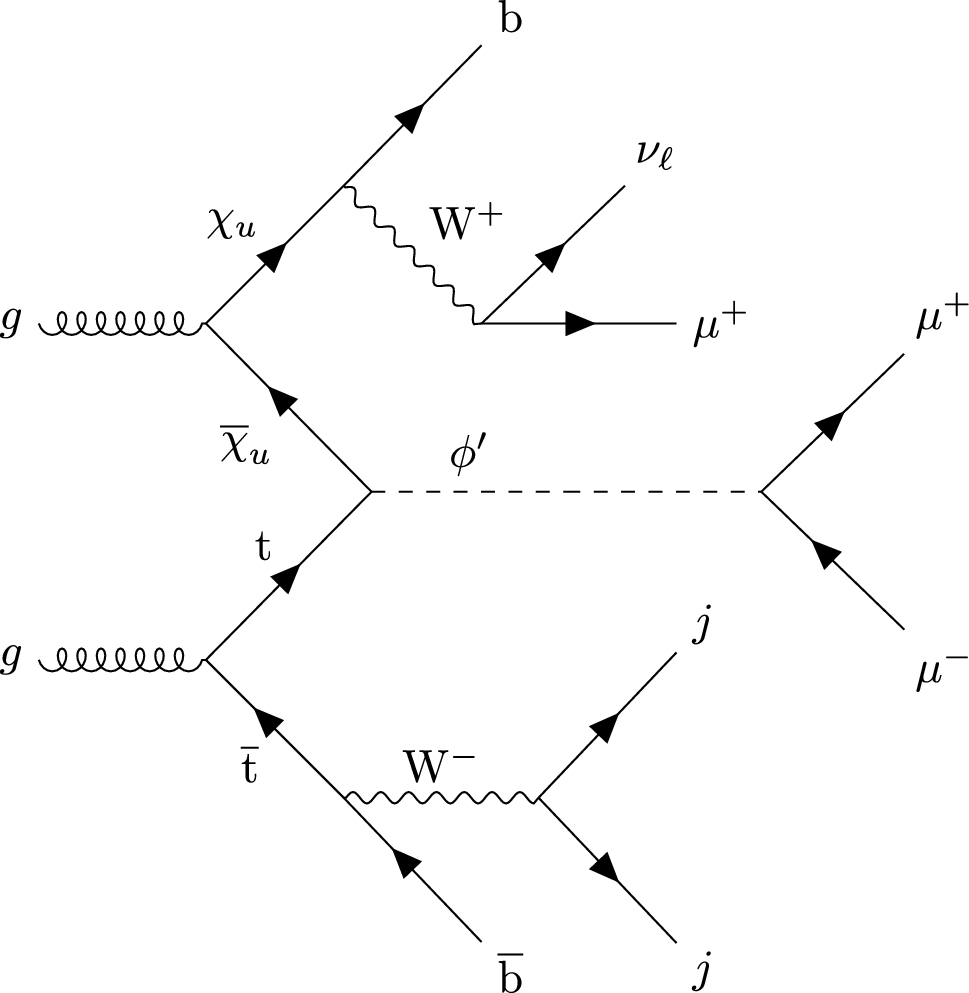
\includegraphics[width=0.5\textwidth]{main_channel.png}
	\end{center}
	The $\phi'$ decays to a pair of muons, the top quark decays fully hadronically, and the $\chi_\mathrm{u}$ decays semi-leptonically to muons, neutrinos and $b$-jets.
\end{frame}
\begin{frame}{Feasible Experimental Signatures}{Search Channel}
	Representative Feynman diagram for the production of a $\phi'$ boson in association with a $\chi_\mathrm{u}$ vector-like quark through the fusion of a gluon pair from incoming protons.
	\begin{center}
		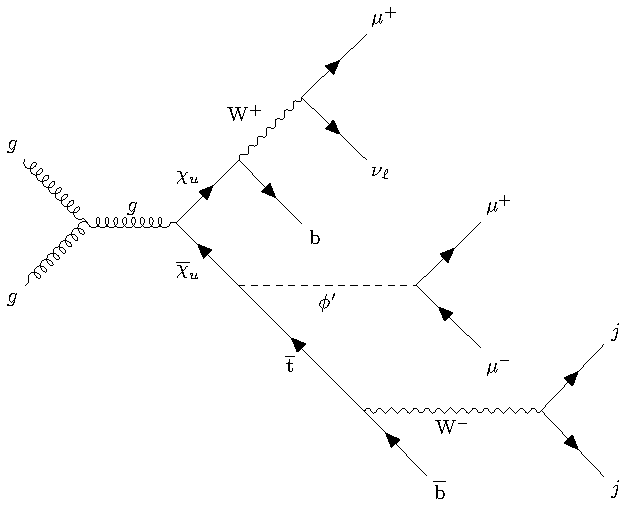
\includegraphics[width=0.6\textwidth]{signal_ggfusion.pdf}
	\end{center}
	The $\phi'$ decays to a pair of muons, the top quark that decays fully hadronically, and the $\chi_\mathrm{u}$ decay semi-leptonically to muons, neutrinos and jets.
\end{frame}

\begin{frame}{Feasible Experimental Signatures}{Cross Section}
	\begin{figure}
    \centering
    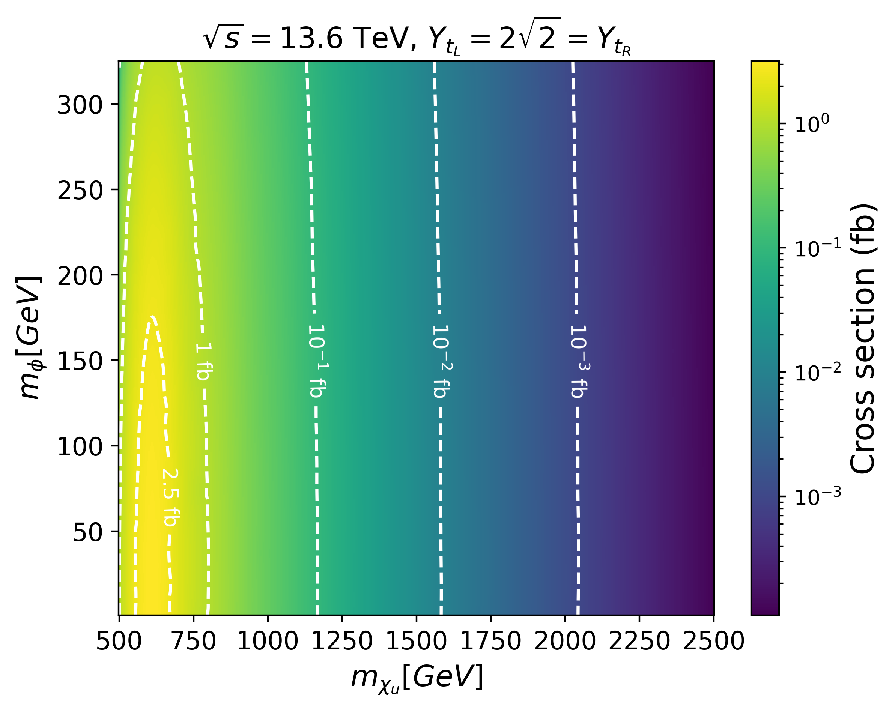
\includegraphics[width=.7\linewidth]{cross_section_by_masses.pdf}
    \caption{Projected cross section (fb) plot for $pp\to t \chi_\mathrm{u} \phi'$ and subsequent decay as a function of $m(\chi_\mathrm{u})$ and $m(\phi')$.}
    \label{fig:xs-plot}
\end{figure}

\end{frame}

\begin{frame}{Feasible Experimental Signatures}{Background}
	Representative Feynman diagram for a background event. A $Z$ boson is produced in association with a top quark through the fusion of a top, anti top pair from incoming protons. 
	\begin{center}
		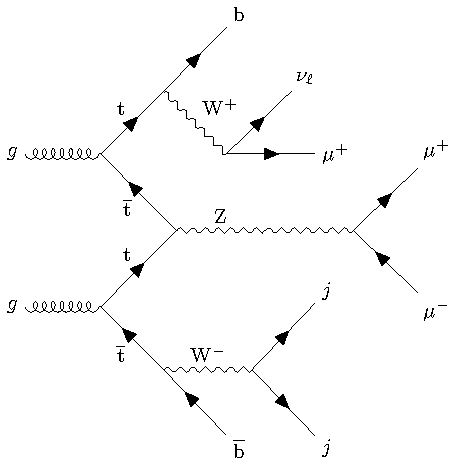
\includegraphics[width=0.45\textwidth]{bg_Z_full.pdf}
	\end{center}
	The $Z$ boson subsequently decays to a pair of muons and the two spectator top quarks decay semi-leptonically and purely hadronically to muons, neutrinos and jets, resulting in the same final states as the signal event.
\end{frame}

\begin{frame}{Feasible Experimental Signatures}{Kinematic Variables}
	\begin{figure}
	\centering
	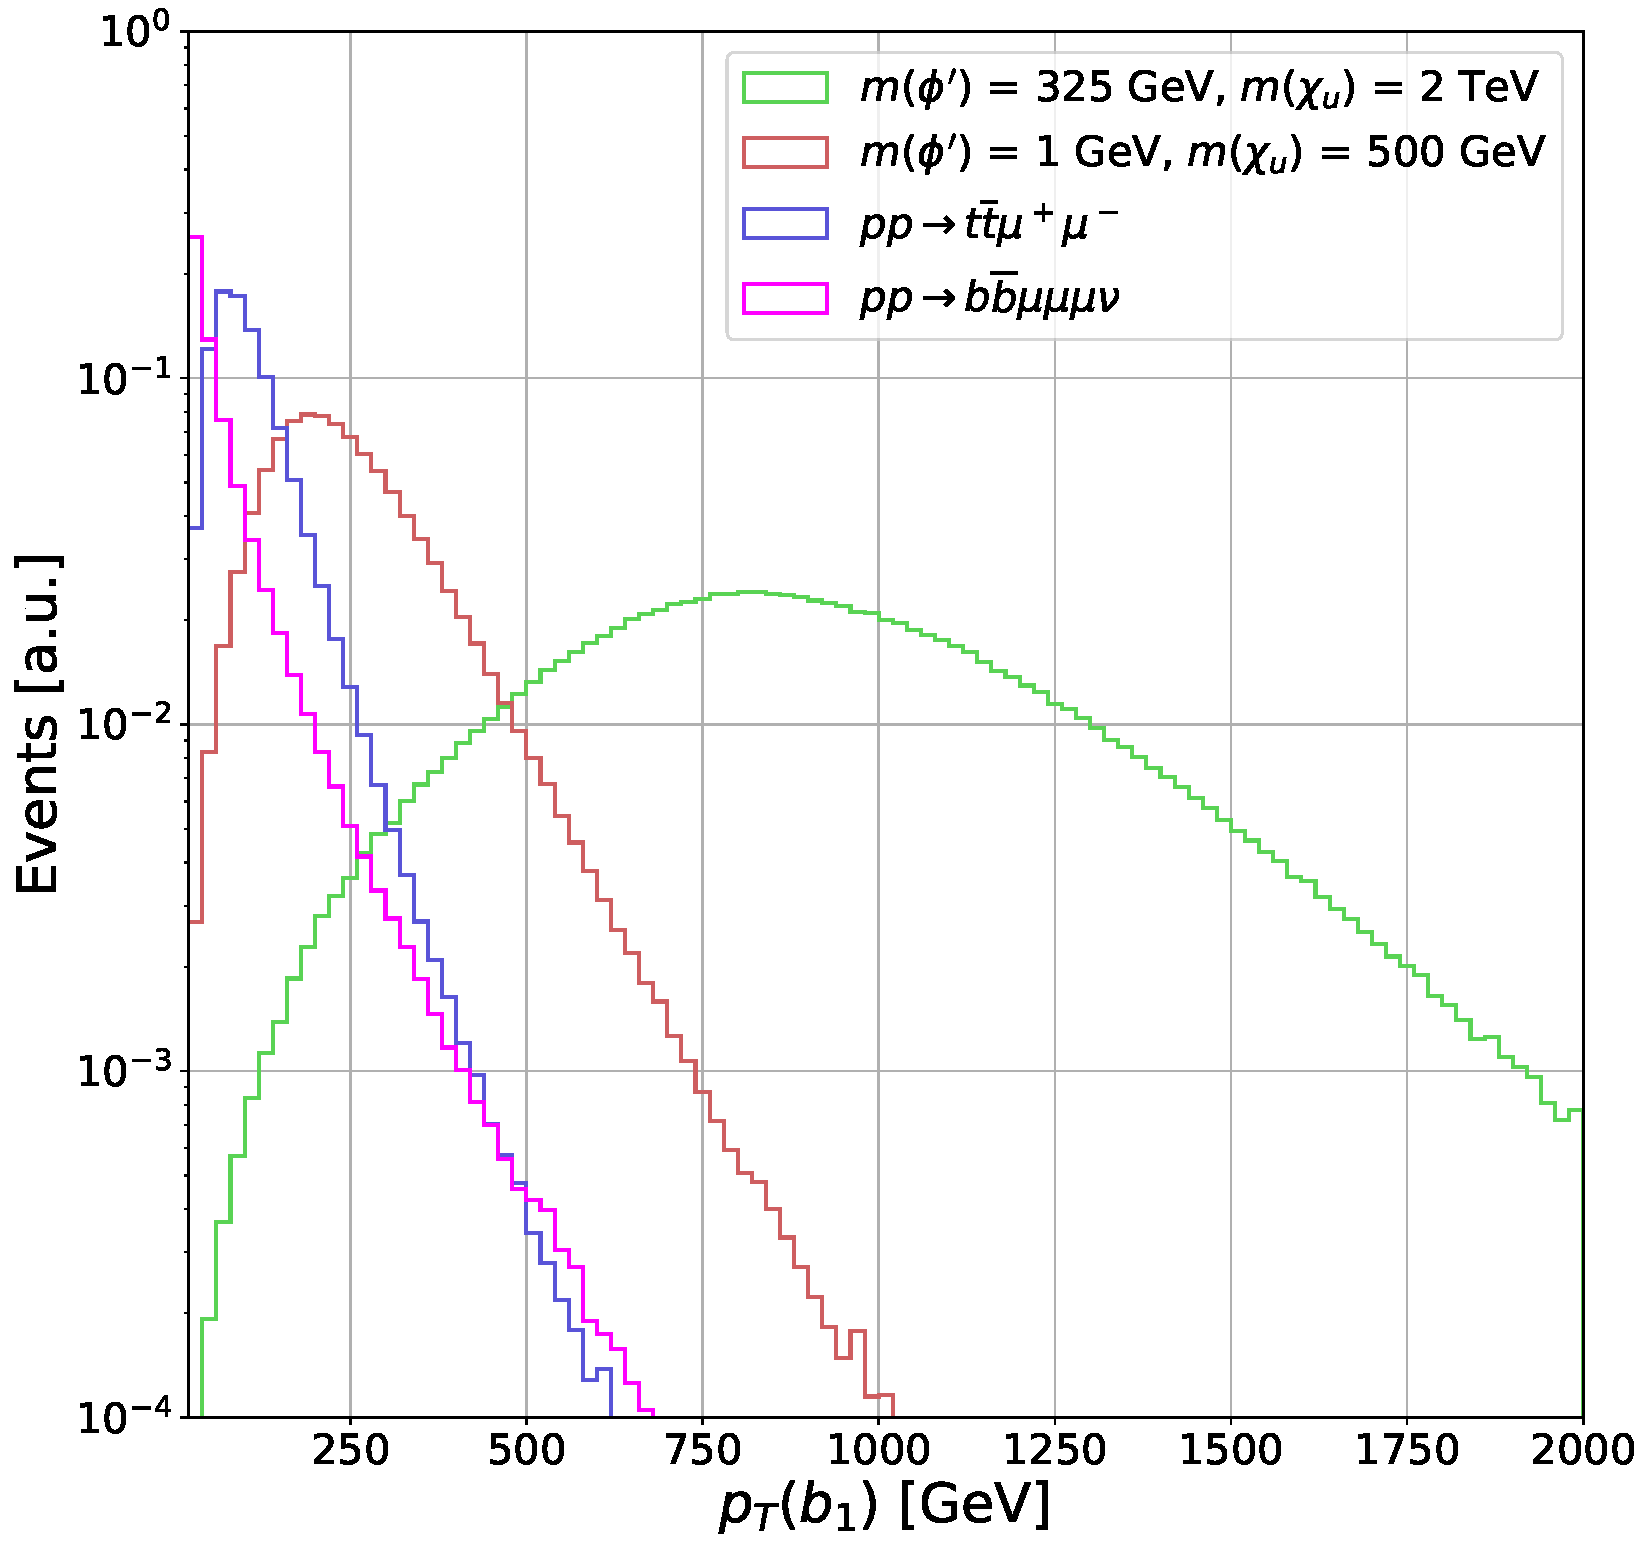
\includegraphics[width=.6\linewidth]{PT_b1.pdf}
	\caption{Transverse momentum distribution of the leading \textrm{b}-quark jet candidate. The distributions are shown for the two main SM background processes and two signal benchmark points.\label{fig:pTb1}}
	\end{figure}
\end{frame}

\begin{frame}{Feasible Experimental Signatures}{Kinematic Variables}
	\begin{figure}
	\centering
	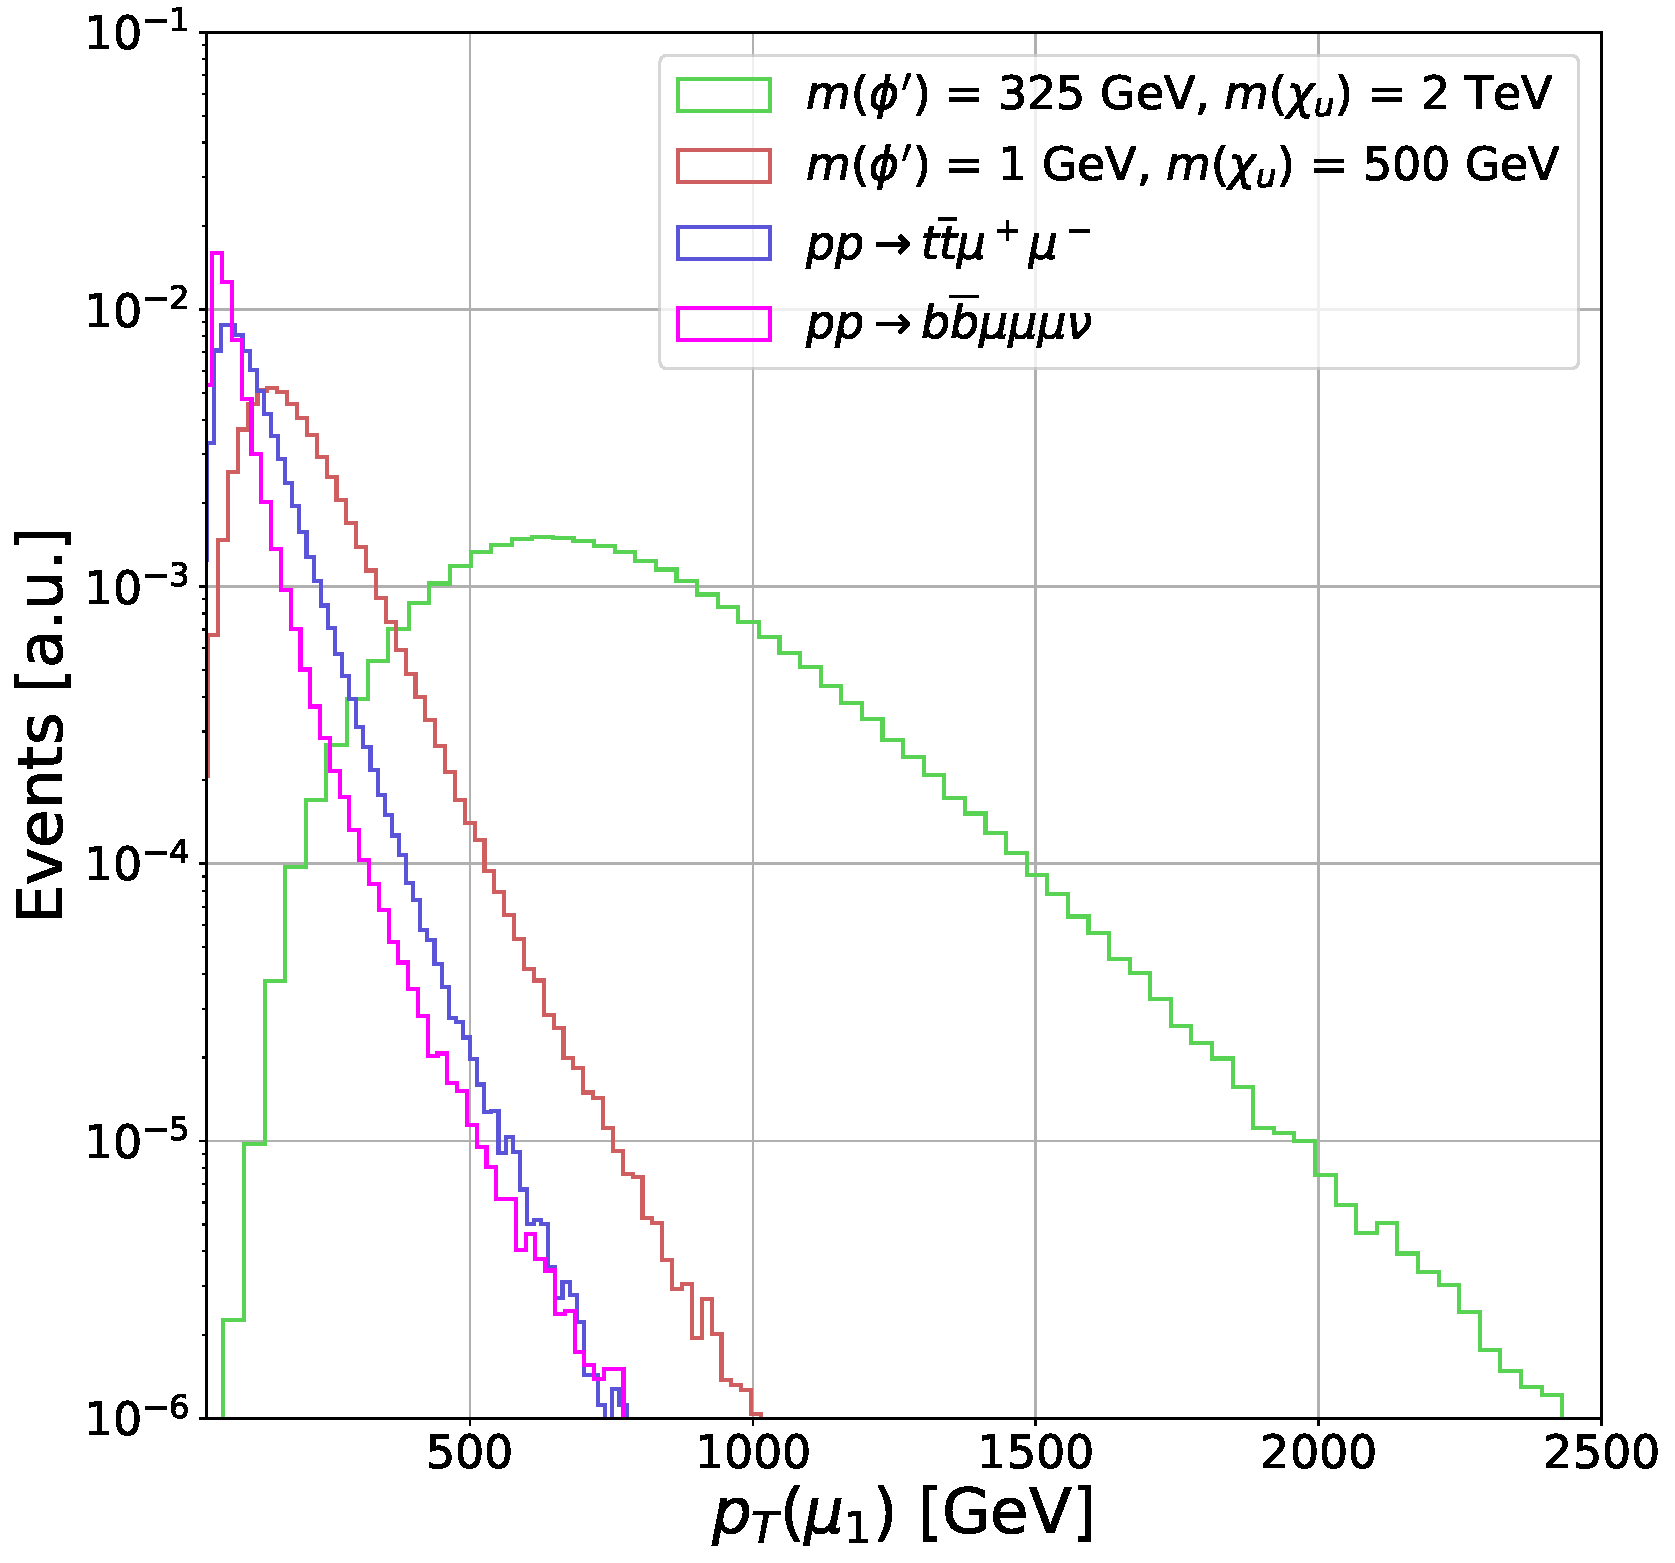
\includegraphics[width=.6\linewidth]{PT_mu1_1.pdf}
	\caption{Transverse momentum distribution of the leading muon candidate. The distributions are shown for the two main SM background processes and two signal benchmark points.\label{fig:pTmu1}}
	\end{figure}
\end{frame}

\begin{frame}{Feasible Experimental Signatures}{Kinematic Variables}
	\begin{figure}
	\centering
	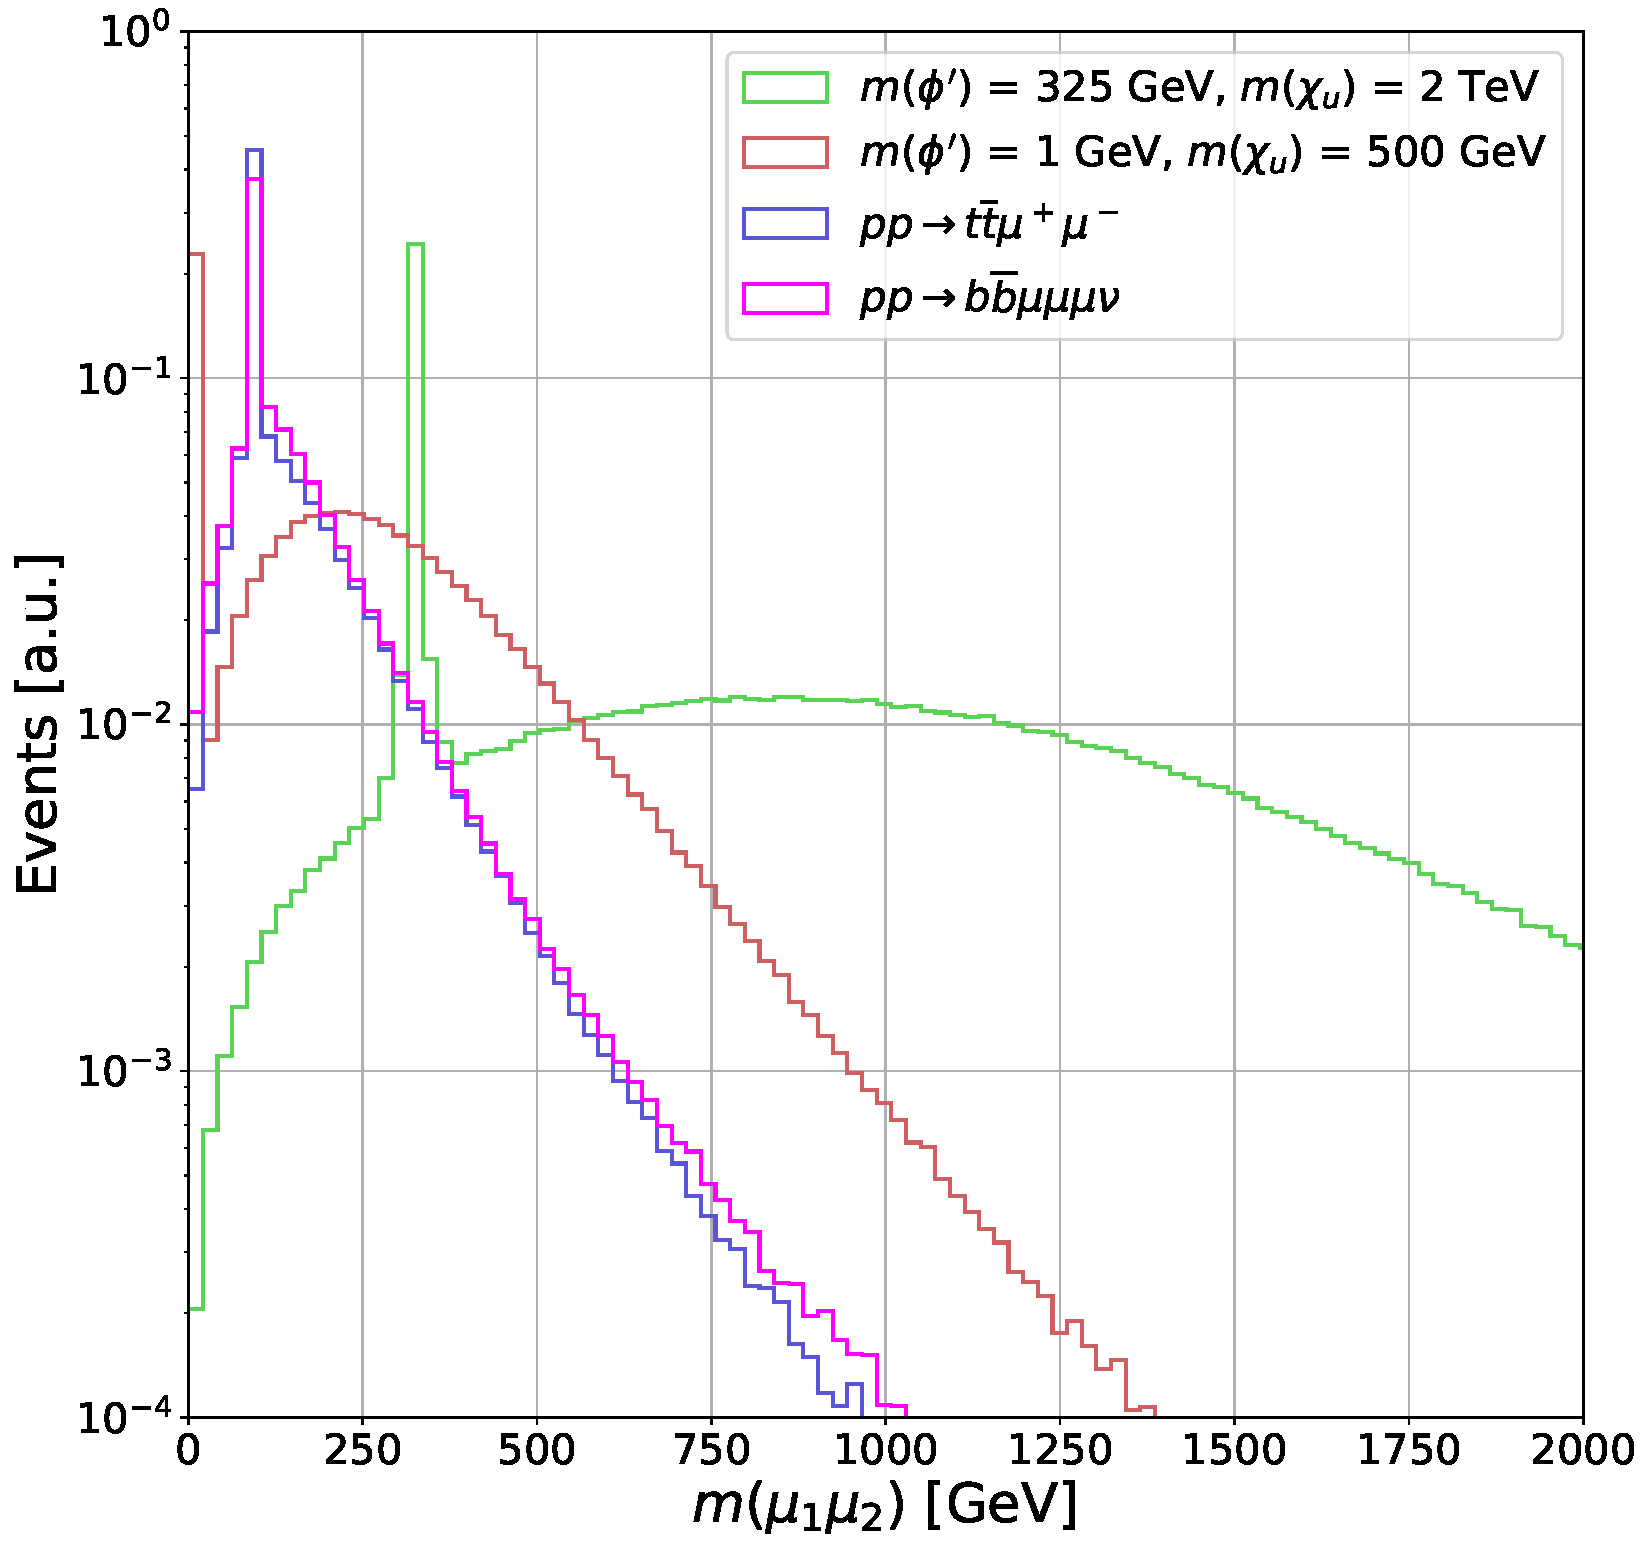
\includegraphics[width=.6\linewidth]{M_mu_1_2.pdf}
	\caption{Invariant mass distribution of the muon pair with the highest and second highest transverse momentum. The distributions are shown for the two main SM background processes and two signal benchmark points.\label{fig:_mu12}}
	\end{figure}
\end{frame}




\begin{frame}{Feasible Experimental Signatures}{Gradient Boosting}
	\begin{figure}
		\centering
		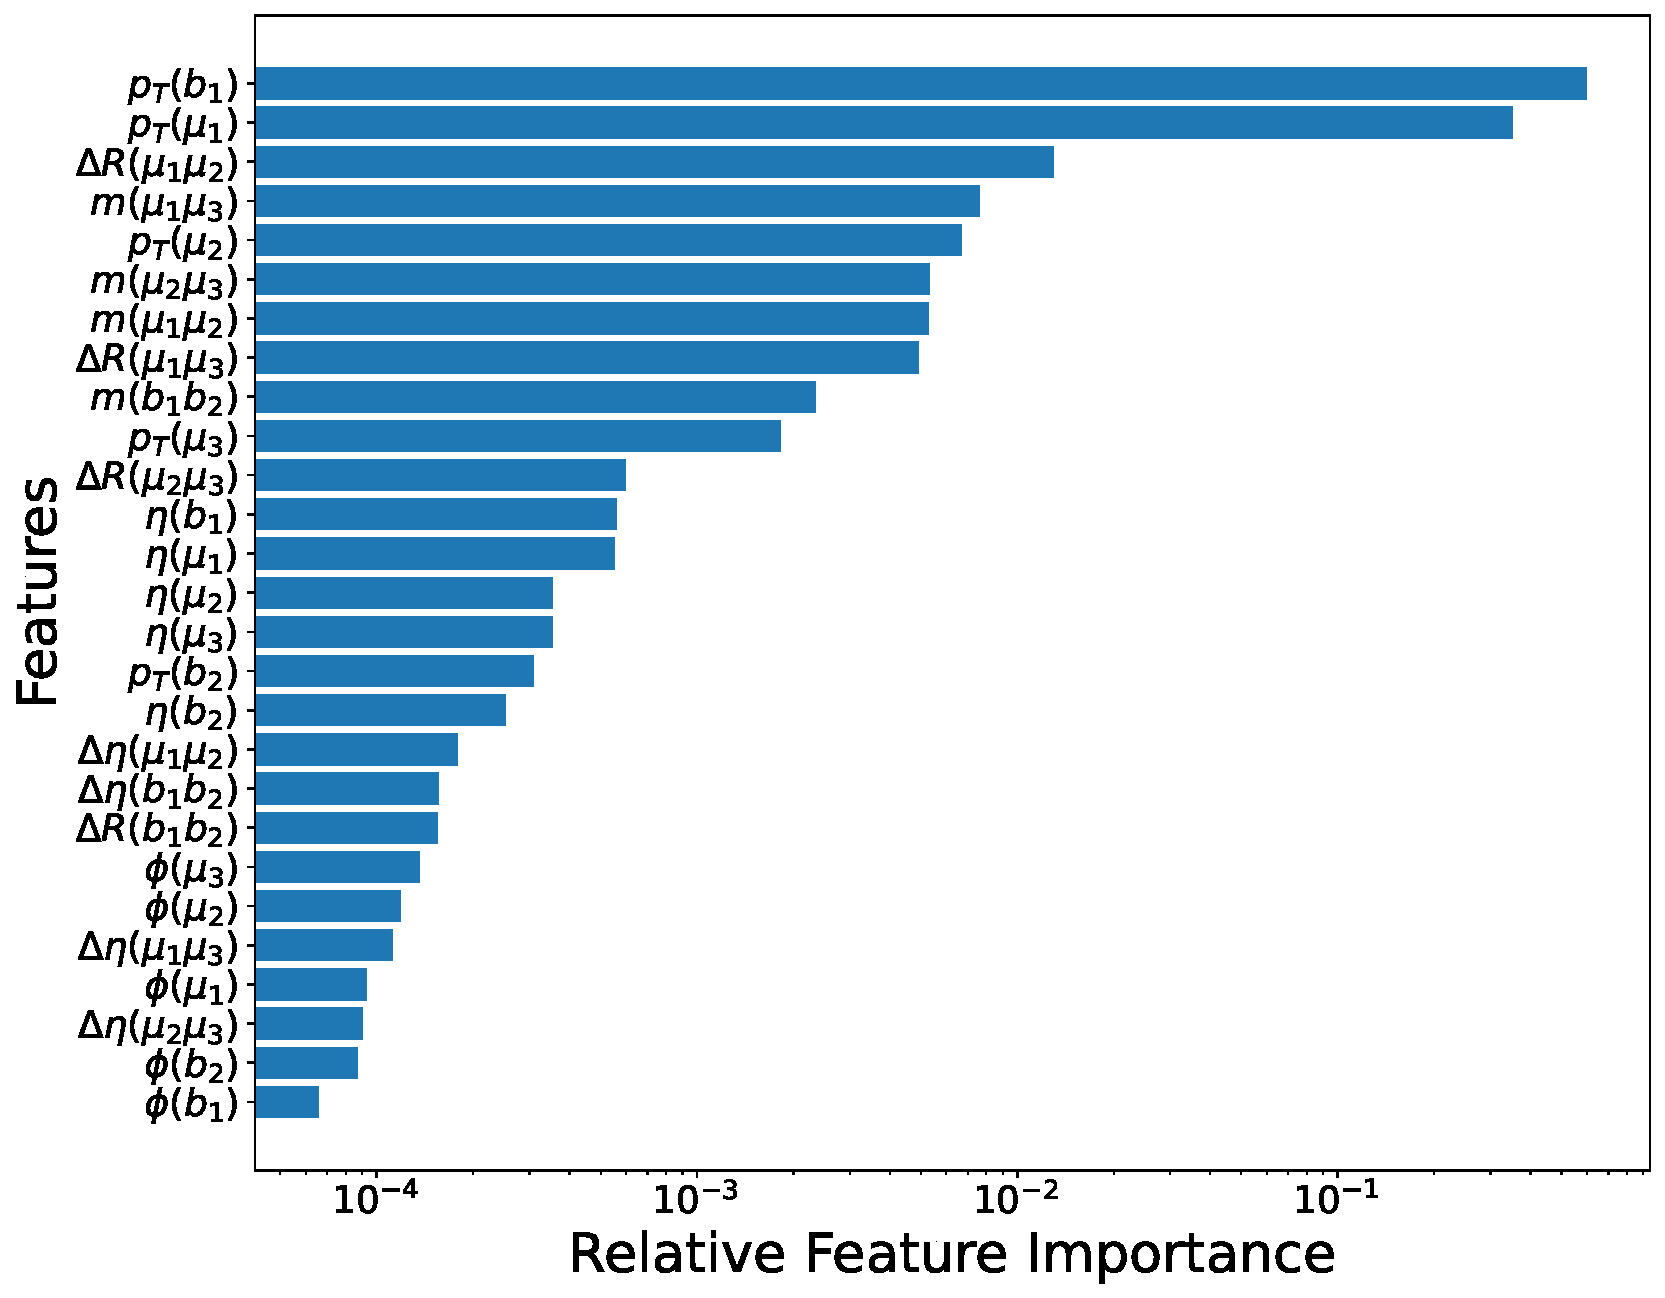
\includegraphics[width=.6\linewidth]{feature_importance.pdf}
		\caption{Relative importance of features in training for a benchmark signal scenario with $m(\phi')=325\, \mathrm{GeV}$ and $m(\chi_\mathrm{u})=2000\, \mathrm{GeV}$.}
		\label{fig:feature_importance}
	\end{figure}
	
\end{frame}

\begin{frame}{Feasible Experimental Signatures}{Gradient Boosting}
	\begin{figure}
	\centering
		\centering  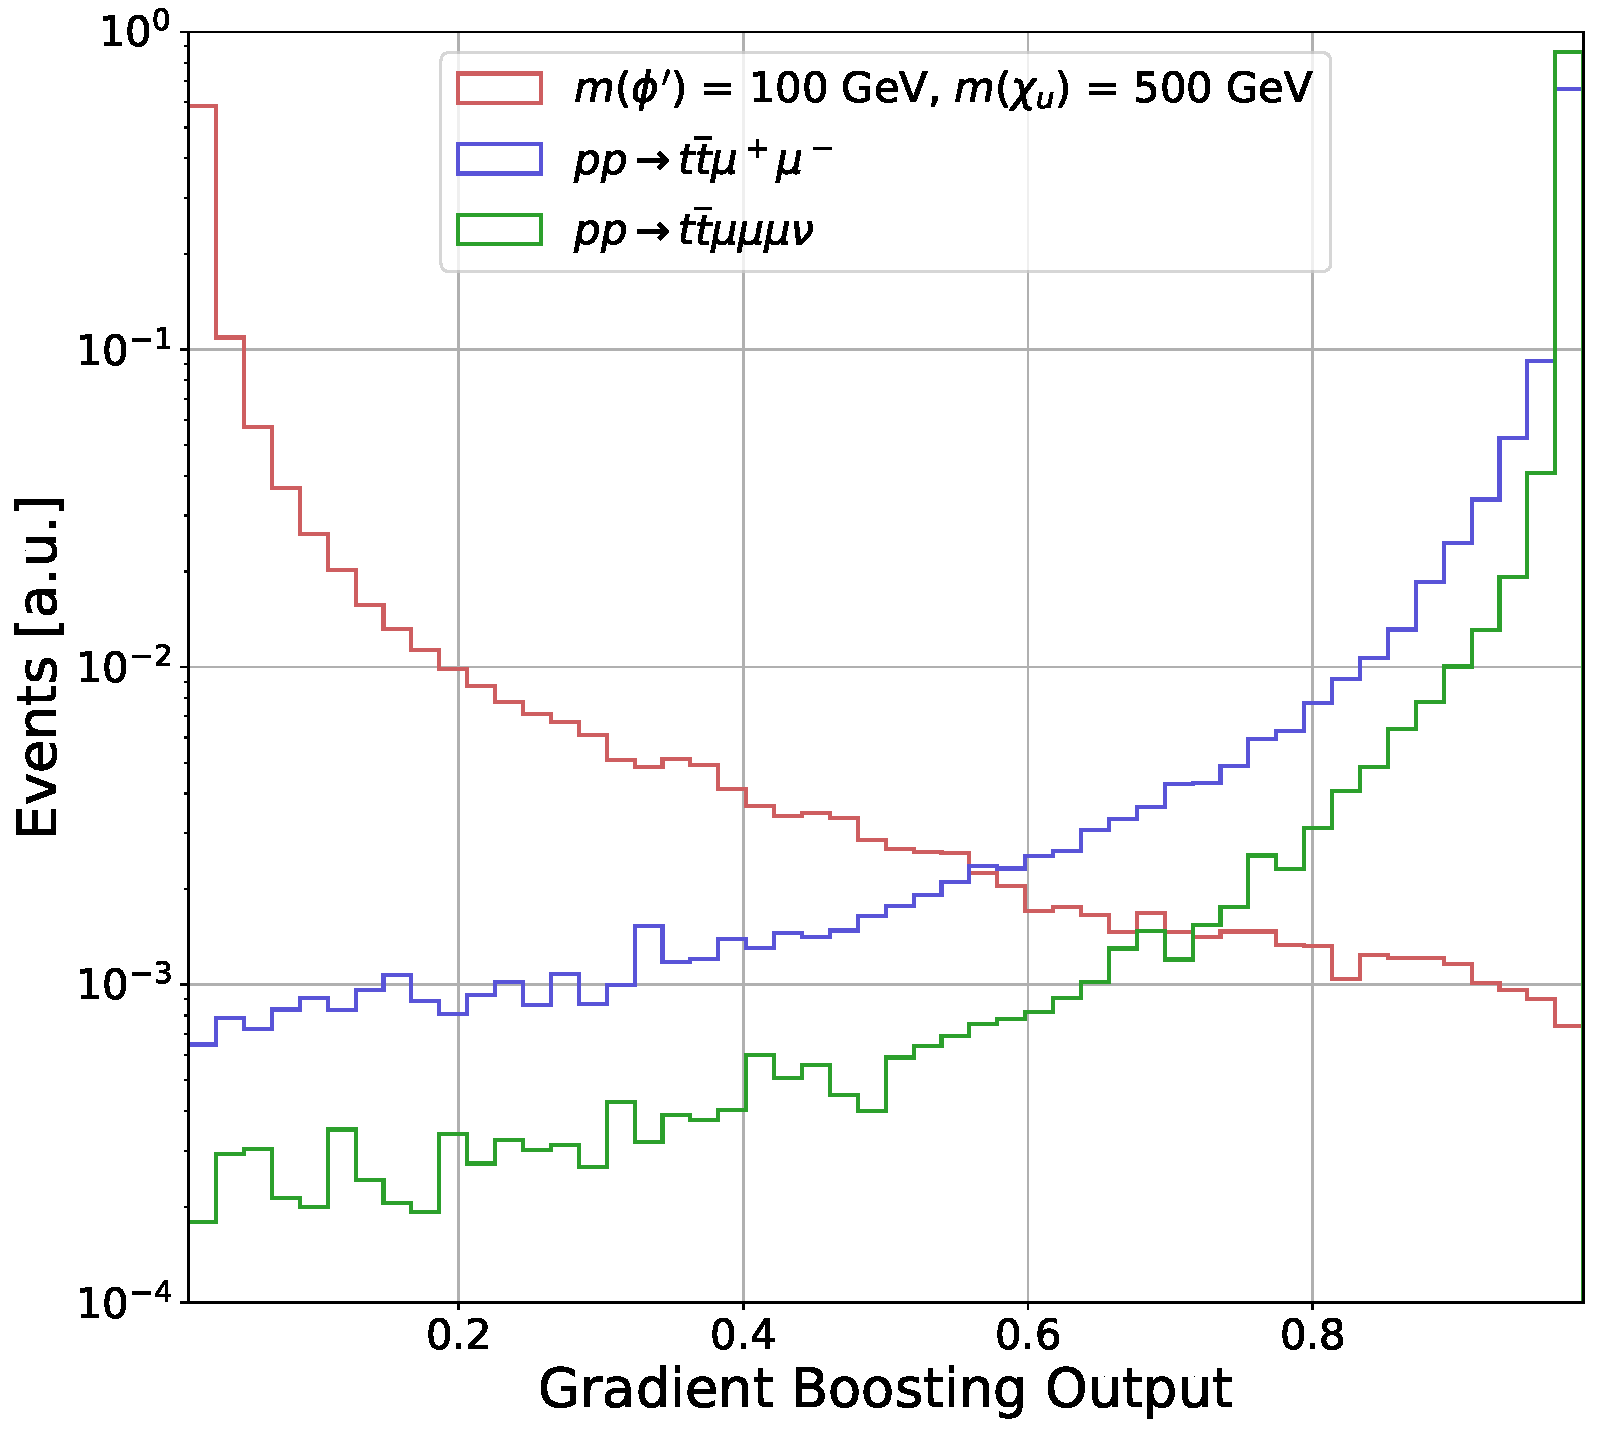
\includegraphics[width=.6\linewidth]{XGB_output.pdf}
		\caption{Output of the gradient boosting algorithm for a benchmark $m(\phi') = 100$~\textrm{GeV} and $m(\chi_\mathrm{u}) = 500\, \mathrm{GeV}$ signal, and dominant backgrounds. The distributions are normalized to unity.}
		\label{fig:xgboostout}
	\end{figure}
\end{frame}

\begin{frame}{Feasible Experimental Signatures}{Signal Significance}
	\begin{figure}[]
		\centering
		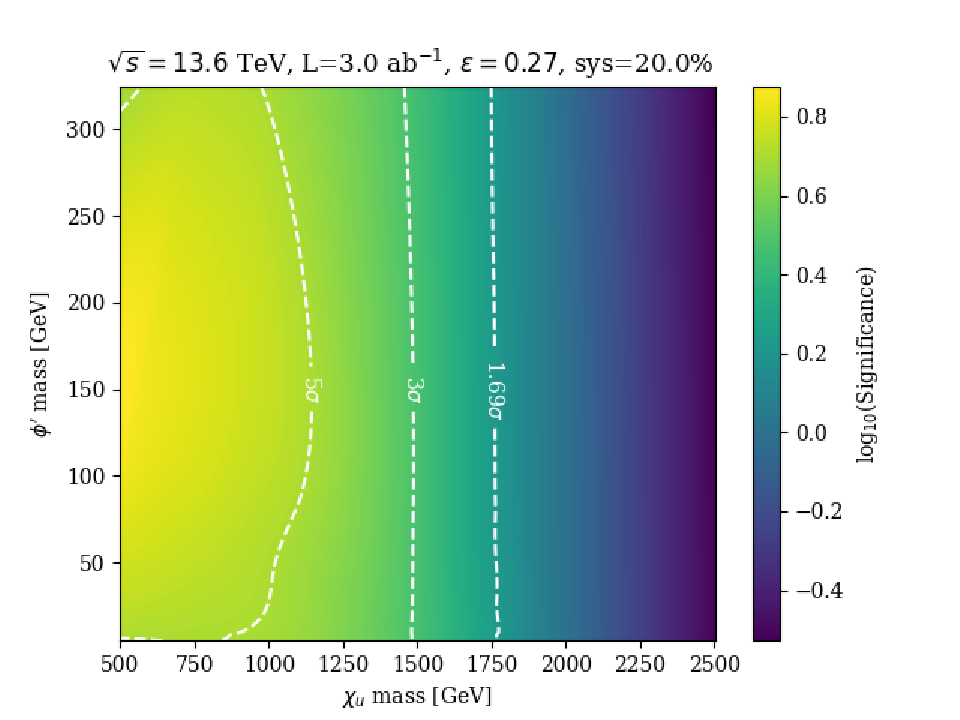
\includegraphics[width=.6\linewidth]{significance.pdf}
		\caption{Signal significance for the high luminosity LHC era, considering with 3000  $\mathrm{fb}^{-1}$ of collected data.}
		\label{fig:/significance_3000}
	\end{figure}
\end{frame}


\begin{frame}{Reference}
	\begin{center}
		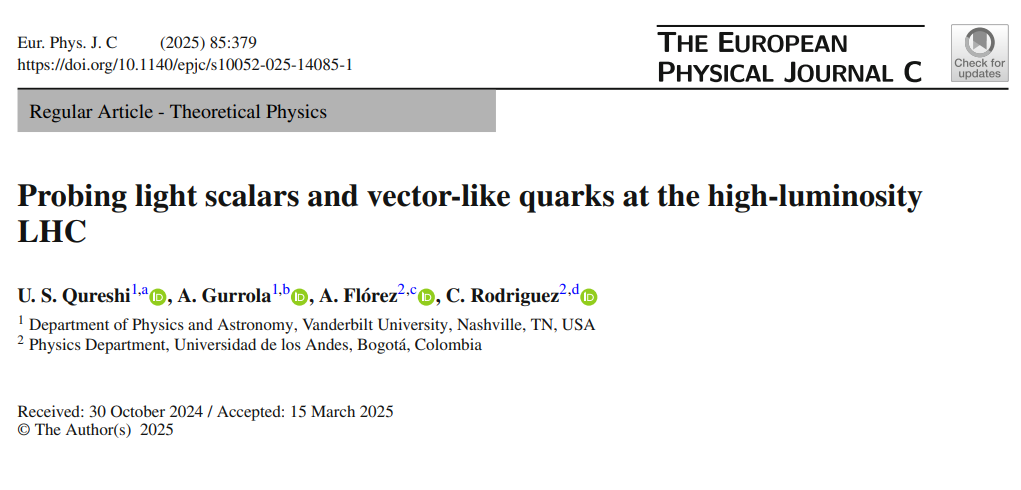
\includegraphics[width=.9\linewidth]{reference.png}
	\end{center}
\end{frame}
\end{document}

